% Stage: 01 入口 ／ 説明用コード: src/stages/01\_mpp/src/ftqc
\chapter{表面符号パッチを作る（MPP）}\label{ch:surface_patch}

\begin{chaptergoal}
  \begin{itemize}
  \item $d=3$ の rotated 表面符号パッチにおけるスタビライザの市松配置と境界規則を、局所 id で列挙できるようになります。
  \item データ量子ビットの支持集合として論理演算子 $X_L$・$Z_L$ を定義し、その重みが符号距離 $d$ に一致することを理解します。
  \item MPP（多体パウリ測定）でアンシラを使わずにスタビライザ測定を模擬する意味と、その限界を理解します。
  \item 一様検出器則にもとづくメモリ実験を実装し、物理誤り率 $p$ に対する論理エラー率のふるまいを観測できるようになります。
  \end{itemize}
\end{chaptergoal}

第6章では Stim の基本操作（\texttt{Circuit}、\texttt{DETECTOR}、検出器誤りモデル、サンプラ、デコーダ呼び出し）を学びました。
本章ではそれらの道具を使い、本書で最初に組み立てる具体的な誤り耐性の対象――$d=3$ の rotated 表面符号 1 パッチ――を、\textbf{MPP}（Multi-body Pauli Product measurement、多体パウリ測定）という現象論的な近似で作ります。
MPP は、本来アンシラと \texttt{CX} 列を介して行うスタビライザ測定を、Stim 上で 1 命令の多体パウリ測定として直接模擬する機能です。
アンシラの配線やスケジューリングを後回しにできるので、まずは「どのスタビライザをどの順番で測り、どの検出器則を張るか」という幾何とロジックだけに集中できます。
この単純化こそが Stage 01（第 III 部）の入口である本章の狙いであり、対応する説明用コードは \codepath{src/stages/01_mpp/src/ftqc/surface_patch.py} です。

\begin{notebox}
  Stage: \textbf{01}。
  説明用コードは主に \codepath{src/stages/01_mpp/src/ftqc/surface_patch.py}（および \codepath{src/stages/01_mpp/src/ftqc/geom_lattice_surgery.py} の幾何列挙ロジック）です。
  アンシラベースの \texttt{CX} スケジュールや回路レベルの厳密な距離解析には踏み込みません（第14–15章）。
\end{notebox}

\section{d=3 パッチのスタビライザ列挙}\label{sec:stab_enum}

\subsection{市松配置}

本章で採用する奇数距離の rotated 表面符号パッチは、$d\times d$ 個のデータ量子ビットを格子状に並べ、その隙間にスタビライザ（プラケット）を市松模様に配置します\cite{fowler2012surface}。
$d=3$ では 9 個のデータ量子ビットを使い、本章では行列位置 $(r,c)\in\{0,1,2\}^2$ に対して
\begin{equation}
  \mathrm{id} = 3r + c
\end{equation}
という\textbf{ローカル id} を割り当てます（\codepath{src/stages/01_mpp/src/ftqc/surface_patch.py} の \texttt{SurfacePatch} が採用する規約です）。
座標としては $(2c+1,\,2r+1)$ を対応させ、プラケット中心 $(c_x,c_y)$ の型は
\begin{equation}
  \mathrm{type}(c_x,c_y) = \begin{cases} Z & \left(\dfrac{c_x+c_y}{2}\right) \bmod 2 = 0\\ X & \text{それ以外} \end{cases}
\end{equation}
という市松規則で決まります（\codepath{src/stages/01_mpp/src/ftqc/geom_lattice_surgery.py} の \texttt{\_dtype} が一般のセル集合に対してこの規則を実装しています）。
4 隅すべてがデータで埋まっていれば重み 4 のバルクスタビライザに、パッチの外周では 2 隅だけが埋まる重み 2 の境界スタビライザになります。

\subsection{境界}

境界では、市松規則をそのまま使うと\textbf{上下境界には $X$ 型、左右境界には $Z$ 型}の重み 2 スタビライザだけが残ります（\texttt{\_stabs} が「上下境界なら $X$、左右境界なら $Z$」という条件で採用/不採用を判定しています）。
この非対称性は偶然ではなく、後述する論理演算子 $X_L$・$Z_L$ の向きと整合するように選ばれています。

図~\ref{fig:d3_patch} に $d=3$ パッチの全体像を示します。
円がデータ量子ビット（ローカル id）、正方形がスタビライザ（バルクは重み 4、境界は重み 2）です。

\begin{figure}[htbp]
  \centering
  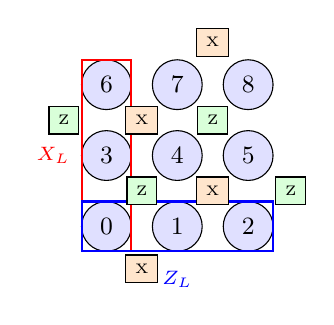
\begin{tikzpicture}[font=\small, scale=0.9]
    \foreach \id/\c/\r in {0/0/0,1/1/0,2/2/0,3/0/1,4/1/1,5/2/1,6/0/2,7/1/2,8/2/2}{
      \node[circle,draw,fill=blue!12,minimum size=18pt,inner sep=0pt] at (\c,\r) {\id};
    }
    \draw[thick,red] (-0.35,-0.35) rectangle (0.35,2.35);
    \node[red] at (-0.75,1) {\scriptsize $X_L$};
    \draw[thick,blue] (-0.35,-0.35) rectangle (2.35,0.35);
    \node[blue] at (1,-0.75) {\scriptsize $Z_L$};
    \node[draw,fill=green!15] at (0.5,0.5) {\tiny Z};
    \node[draw,fill=orange!20] at (1.5,0.5) {\tiny X};
    \node[draw,fill=orange!20] at (0.5,1.5) {\tiny X};
    \node[draw,fill=green!15] at (1.5,1.5) {\tiny Z};
    \node[draw,fill=orange!20] at (0.5,-0.6) {\tiny X};
    \node[draw,fill=orange!20] at (1.5,2.6) {\tiny X};
    \node[draw,fill=green!15] at (-0.6,1.5) {\tiny Z};
    \node[draw,fill=green!15] at (2.6,0.5) {\tiny Z};
  \end{tikzpicture}
  \caption{$d=3$ rotated 表面符号パッチの市松配置。円はデータ量子ビット（ローカル id $=3r+c$）、正方形はスタビライザ（バルク重み4／境界重み2）。赤枠が $X_L$（左列 $\{0,3,6\}$）、青枠が $Z_L$（下行 $\{0,1,2\}$）。}
  \label{fig:d3_patch}
\end{figure}

\subsection{geom\_lattice\_surgery / mpp 内の列挙ロジック}

\codepath{src/stages/01_mpp/src/ftqc/surface_patch.py} は、上の幾何・境界規約で決まる独立な 8 個のスタビライザを \texttt{GEOM\_STABS\_D3} という定数リストとして直接持っています。

\begin{lstlisting}[caption={$d=3$ パッチのスタビライザ列挙（\codepath{src/stages/01_mpp/src/ftqc/surface_patch.py}）},label=lst:geom_stabs_d3]
GEOM_STABS_D3 = [
    ("X", [0, 1]),       ("Z", [0, 1, 3, 4]),
    ("X", [1, 2, 4, 5]), ("Z", [2, 5]),
    ("Z", [3, 6]),       ("X", [3, 4, 6, 7]),
    ("Z", [4, 5, 7, 8]), ("X", [7, 8]),
]
\end{lstlisting}

同じファイルの \texttt{SurfacePatch} クラスは、この静的なリストを\textbf{自明に信用せず}、Stim 組み込みの \texttt{surface\_code:rotated\_memory\_z} 回路（アンシラベース、まだこの章では踏み込みません）を生成し、その \texttt{CX} スケジュールから逆に「どのアンシラがどのデータ集合を測っているか」を \texttt{\_extract\_stabilizers} で復元して、\texttt{GEOM\_STABS\_D3} と一致することを検証しています。
本章で必要なのは、幾何的な列挙（市松＋境界規則）と Stim の実装が一致しているという\textbf{事実}だけで、アンシラ側の \texttt{CX} スケジュールの詳細（第14–15章の主題）ではありません。
実際に確認すると、\texttt{SurfacePatch(3).stabilizers} は \texttt{GEOM\_STABS\_D3} と要素ごとに一致します。

\section{論理 \texorpdfstring{$X_L$・$Z_L$}{X\_L・Z\_L} とデータ/アンシラ}\label{sec:logical_ops}

\subsection{論理演算子の代表元}

$X_L$・$Z_L$ は、いずれのスタビライザとも可換でありながらスタビライザ群には含まれない演算子、すなわちパウリ群内の中心化群（慣例的には正規化群）の剰余類の代表元として選びます\cite{gottesman1997stabilizer}。
\texttt{SurfacePatch} では、図~\ref{fig:d3_patch} の左列を $X_L$、下行を $Z_L$ の代表元に採っています。

\begin{lstlisting}[caption={論理演算子の支持集合（\codepath{src/stages/01_mpp/src/ftqc/surface_patch.py} の \texttt{SurfacePatch.\_\_init\_\_}）},label=lst:xl_zl]
# 論理演算子: XL=左列(x=1), ZL=下行(y=1)
self.XL = sorted(self.stim2local[q] for q, c in self.data.items() if c[0] == 1)
self.ZL = sorted(self.stim2local[q] for q, c in self.data.items() if c[1] == 1)
\end{lstlisting}

これにより \texttt{XL == [0, 3, 6]}、\texttt{ZL == [0, 1, 2]} となり、いずれも重み $3=d$ の一列（一行）です。
重みが符号距離 $d$ に一致するのは偶然ではなく、$d$ とは「ある論理状態を別の論理状態へ変える最小の誤りの個数」（第3章）そのものだからです。
左列の $X$ 鎖は $X_L$、下行の $Z$ 鎖は $Z_L$ を実装し、全スタビライザと可換なまま相補的な論理値を反転します。$Y$ 鎖は $X$ 成分と $Z$ 成分を同時に持つため、任意の列へ置いたものが同じ性質を持つとは限りません。

\subsection{メモリの向き}

本章で使うメモリ実験は\textbf{$Z$ 基底メモリ}です。
データ量子ビットを $\ket{0}^{\otimes 9}$（$Z$ 固有状態）に初期化し、スタビライザ測定を何ラウンドか繰り返した後、最終的に $Z_L$ を読み出します。
この向きが重要なのは、初期状態が $Z$ 固有状態であるために\textbf{ラウンド0では $Z$ 型スタビライザだけが決定論的}になり、$X$ 型スタビライザは初期化直後には値が定まっていない、という非対称性が生じる点です（次節の検出器則に直結します）。
これは Stim 側のタスク名 \texttt{surface\_code:rotated\_memory\_z} の「\texttt{\_z}」が指す向きと同じです。
逆向きの $X$ 基底メモリも同じ幾何で対称的に作れますが、本章の中心である \texttt{mpp\_memory\_logical\_error}（次節）は $Z$ 基底メモリのみをハードコードしています。これは意図的な単純化であり、$X$ 基底版は同じ考え方を左右対称に適用すれば作れます。

\subsection{データ量子ビットだけで構成する理由}

第3章で確認したとおり、シンドローム測定は本来\textbf{アンシラを介した間接測定}です。
しかし MPP を使う本章の構成には、物理的なアンシラ量子ビットが 1 個も現れません。
これは MPP が「複数データ量子ビットにまたがる多体パウリ演算子を、Stim の内部でアンシラなしに直接測定する」という\textbf{理想化された命令}だからです。
実機ではこの多体測定を、補助量子ビットと \texttt{CX} 列で段階的に構成する必要があります（第14章以降）。
本章では、その配線の詳細をいったん脇に置き、「どの多体パウリをいつ測るか」という幾何とロジックだけを先に固めます。

\section{スタビライザ測定とノイズ（MPP）}\label{sec:mpp_noise}

\subsection{MPP の意味（現象論）}

Stim の \texttt{MPP} 命令は、\texttt{stim.target\_x}／\texttt{target\_z} と \texttt{stim.target\_combiner()} を組み合わせることで、互いに可換な多体パウリ積を測定命令として指定できます\cite{gidney2021stim,stim2026python}。
\codepath{src/stages/01_mpp/src/ftqc/surface_patch.py} の \texttt{mpp\_memory\_logical\_error} は、この命令を使って \texttt{GEOM\_STABS\_D3} の 8 個のスタビライザを毎ラウンド直接測定します。

\begin{lstlisting}[caption={MPP によるスタビライザ測定（\codepath{src/stages/01_mpp/src/ftqc/surface_patch.py} の \texttt{mpp\_memory\_logical\_error} を抜粋）},label=lst:mpp_measure]
for rnd in range(rounds + 1):
    c.append("DEPOLARIZE1", data, p)          # データ量子ビットの脱分極誤り
    for si, (t, sup) in enumerate(sp.stabilizers):
        tg, first = [], True
        fn = {"X": stim.target_x, "Z": stim.target_z}
        for q in sup:
            if not first:
                tg.append(stim.target_combiner())
            tg.append(fn[t](q))
            first = False
        c.append("MPP", tg, p)                # 多体パウリ測定自体にも誤り率 p
\end{lstlisting}

ここでノイズは 2 か所に入っています。
\texttt{DEPOLARIZE1(data, p)} はラウンドごとにデータ量子ビットが受ける物理誤りで、これは第3章の「反復符号でビットが確率 $p$ で反転する」に対応する現象論的ノイズです。
一方 \texttt{MPP(tg, p)} の第 2 引数 \texttt{p} は、測定そのものが確率 $p$ で誤った結果を返すという抽象化で、アンシラ経由の測定で本来起きる測定誤り・伝播誤りをひとまとめに近似したものです。
これは Stim が提供する現象論ノイズモデルの標準的な使い方であり、実際のゲート単位の誤り伝播（第14章以降の回路レベルノイズ）とは異なる、より粗い近似であることを明示しておきます。

\subsection{一様検出器則の導入}

アンシラを使わない MPP では、同じスタビライザを毎ラウンド同じ添字 \texttt{si} で測り続けるため、検出器則は非常に単純になります。
「同じ添字のスタビライザを、直前ラウンドの測定値と比較する」という\textbf{一様規則}だけで済みます。

\begin{lstlisting}[caption={一様検出器則（\codepath{src/stages/01_mpp/src/ftqc/surface_patch.py} の \texttt{mpp\_memory\_logical\_error} を抜粋）},label=lst:uniform_detector]
if si in prev:
    dets.append([mc, prev[si]])   # 直前ラウンドの同じスタビライザと比較
elif t == "Z":
    dets.append([mc])            # ラウンド0は Z 型のみ単独で決定論的
prev[si] = mc
\end{lstlisting}

ラウンド 0 では、初期状態が $Z$ 固有状態であるために $Z$ 型スタビライザだけが単独で決定論的検出器になり、$X$ 型スタビライザは「まだ比較対象がない」ので検出器を張りません。
ラウンド 1 以降はすべてのスタビライザについて「今回の値 XOR 前回の値」を検出器にします。
最後に $Z_L$ を直接 \texttt{MPP} で測定し、観測量として登録します。
このシンプルさは MPP という理想化の恩恵であり、アンシラ回路ではスタビライザの支持集合自体は変わらなくても、測定順序に依存した\textbf{フック誤り}が絡んでくるため、検出器則の導出はもう一段階複雑になります（第14–15章）。

\section{メモリ実験と論理エラー率}\label{sec:memory_exp}

\subsection{shots}

\codeinline{mpp_memory_logical_error(p, rounds=3, shots=40000)} は、上記の回路を \codeinline{compile_detector_sampler().sample(shots, separate_observables=True)} で多数回サンプリングし、\texttt{pymatching.Matching} でデコードした予測と実際の観測量との XOR の平均を論理エラー率として返します。
\texttt{shots} を増やすほどモンテカルロ推定の統計誤差が小さくなります。真の論理エラー率を $p_L$、ショット数を $N$ とすると、標本比率の標準誤差はおおよそ $\sqrt{p_L(1-p_L)/N}$ です。したがって 4 万 shots が与える桁数は $p_L$ に依存し、失敗が0件でも誤り率が0と確定するわけではなく、95\% 上限の目安は $3/N$ です。

\begin{lstlisting}[caption={メモリ実験の最小実行例},label=lst:memory_min]
# src/stages/01\_mpp で `uv run` して実行する
from ftqc.surface_patch import mpp_memory_logical_error

for p in (0.0, 0.001, 0.003, 0.005, 0.01):
    err = mpp_memory_logical_error(p, rounds=3, shots=40000)
    print(f"p={p:<6} logical_error_rate={err:.4f}")
\end{lstlisting}

\subsection{$p$ 依存の直感}

上の例を実行すると、おおむね次のような結果が得られます（乱数依存のため実行毎に数値は変動します）。

\begin{lstlisting}[caption={実行例の出力},label=lst:memory_output]
p=0.0    logical_error_rate=0.0000
p=0.001  logical_error_rate=0.0027
p=0.003  logical_error_rate=0.0058
p=0.005  logical_error_rate=0.0125
p=0.01   logical_error_rate=0.0256
\end{lstlisting}

$p=0$ ではこの実行例の観測失敗率が $0$ になり、$p$ を大きくすると期待される論理エラー率は増加する傾向を示します。有限ショットの各推定値は統計揺らぎを持つため、個々の実行結果が厳密に単調になる保証はありません。
第3章・第4章で定式化したとおり、量子符号距離 $d$（非自明な論理演算子の最小重み）に対して、重み $d-1$ 以下の Pauli 誤りはシンドロームを生じるかスタビライザとして自明に作用し、重み $t = \lfloor (d-1)/2 \rfloor$ 以下の任意の Pauli 誤りを訂正できます。
本章でのシミュレーション（\texttt{mpp\_memory\_logical\_error}）は、ランダムに注入される物理誤りに対する論理エラー率の単調性やデコーダの全体的な応答挙動を確認するものであり、個々の誤りに対する訂正半径 $t$ を直接検証する実験ではない点に注意してください。
本章の段階では、この単調性を現象論レベルで確認するだけにとどめます。
物理誤り率としきい値 $p_{\mathrm{th}}$ の関係、符号距離 $d$ を増やしたときのスケーリングといった定量的な議論は、合否基準を厳密に定義する第8章以降の主題です。

\codepath{src/stages/01_mpp/src/ftqc/surface_patch.py} の \texttt{demo()} は、この MPP 版（アンシラなし・直接測定）と、Stim 組み込みのアンシラベース回路（\texttt{SurfacePatch.memory\_circuit} / \texttt{decode}、ともに回路レベル）を同じ $p$ で比較しています。
この実装例では、同じ数値 $p$ でも回路レベル版の方が論理エラー率が高くなる傾向があります。ただし両モデルでは $p$ が付く誤り位置とチャネルの数が異なるため、同じ $p$ は同じ総ノイズ強度を意味しません。この比較は、回路レベル版だけが \texttt{CX} や測定を介する伝播（フック誤り）を表せることを示す定性的な例です\cite{dennis2002topological,fowler2012surface}。

\section{やること・スコープ外}\label{ch7:scope}

\subsection{やること}

\begin{itemize}
  \item 市松配置と境界規則にもとづく $d=3$ パッチのスタビライザ列挙（\texttt{GEOM\_STABS\_D3}、\texttt{SurfacePatch.stabilizers}）。
  \item データ量子ビットの支持集合としての論理演算子 $X_L$・$Z_L$ の定義。
  \item MPP によるアンシラなしのスタビライザ測定と、一様検出器則の導入。
  \item $Z$ 基底メモリ実験の実装と、$p$ に対する論理エラー率の単調な増加傾向の現象論的な確認。
\end{itemize}

\subsection{スコープ外}

\begin{itemize}
  \item アンシラベースの \texttt{CX} スケジュール設計そのもの。本章では \texttt{SurfacePatch} が内部検証のために Stim 組み込み回路を使う場面にだけ触れ、スケジュールの中身には踏み込みません（第14–15章）。
  \item 回路レベルノイズにおける符号距離の厳密な議論（\texttt{shortest\_graphlike\_error} による検証）。本章で確認するのは「ノイズなしで検出器が決定論的になる」という、より弱い条件だけです。
  \item $X$ 基底メモリ実験、複数パッチの格子手術（第9–11章）。
\end{itemize}

\section{合否基準での検証}\label{ch7:verification}

本書全体の合否基準には、\codepath{tests/} や \texttt{ls\_handoff\_shells.py} が実践する次の 2 点があります：本書の非 gauge 回路について検出器が決定論的であること、未分解 DEM の全誤り機構が graphlike などの条件を満たす場合に\textbf{\texttt{shortest\_graphlike\_error} が意図した距離 $d$ に一致}すること。
これらの厳密な定義と検証手順は第8章でまとめて導入します。

本章の段階（Stage 01 入口）でサンプリングにより確認できるのは、$p=0$ で観測した範囲に検出器反転と論理失敗がないという統計的な健全性です。
第7.4節の最小実行例で $p=0$ の標本論理エラー率が $0$ になることだけでは、全検出器・観測量の決定論性の証明にはなりません。厳密な確認には Stim の tableau 解析を用いる DEM 構築などが必要です\cite{gidney2021stim,stim2026python}。
一方 \texttt{shortest\_graphlike\_error} による距離の厳密な検証は、検出器誤りモデル（DEM）を明示的に構築して初めて意味を持つため、その手続きと合否用語の正式な定義は次章に委ねます。

\section{まとめ}\label{ch7:summary}

\begin{itemize}
  \item 本章の $d=3$ rotated 表面符号パッチは、採用した市松配置と境界規約によって重み 4（バルク）・重み 2（境界）の独立なスタビライザ 8 個として列挙されます。
  \item 論理演算子 $X_L$・$Z_L$ は、それぞれ左列・下行というデータ量子ビットの支持集合で代表され、その重みは符号距離 $d$ に一致します。
  \item MPP はアンシラを使わずに多体パウリ演算子を直接測定する理想化であり、スタビライザの幾何と検出器則だけに集中するための現象論的な近似です。
  \item MPP では「同じスタビライザを直前ラウンドと比較する」一様検出器則だけでメモリ実験が組めますが、これはアンシラ回路のフック誤りを無視した楽観的な近似でもあります。
  \item $Z$ 基底メモリ実験では、$p=0$ の標本失敗率が0であることと、$p$ に対する論理エラー率の増加傾向を確認できます。有限ショット結果は統計揺らぎを持ちます。
\end{itemize}

次章では、本章で仮置きにした「決定論性」と「距離」を、\texttt{shortest\_graphlike\_error} や gauge 検出器ゼロという機械的に検証可能な合否基準として正式に定義し、MWPM や BP+OSD によるデコードと結び付けます。

\begin{exercise}
  \begin{enumerate}
    \item 図~\ref{fig:d3_patch} を参考に、ローカル id $4$（中心のデータ量子ビット）が支持集合に含まれるスタビライザをすべて列挙し、その型と重みを答えなさい。
    \item $X_L=\{0,3,6\}$ に $Z$ 誤りを 1 個だけ作用させたとき、\texttt{GEOM\_STABS\_D3} のうちどのスタビライザの測定値が反転するかを求め、その位置から誤りが起きたデータ量子ビットを一意に特定できるかどうかを議論しなさい。
    \item \texttt{mpp\_memory\_logical\_error} の \texttt{DEPOLARIZE1(data, p)} の行を削除（$p=0$ に固定）した場合と、\texttt{MPP(tg, p)} の第 2 引数だけを $0$ にした場合とで、それぞれ論理エラー率がどう変化すると予想されるかを、本章のノイズモデルの説明にもとづいて答えなさい。
    \item 本章の $Z$ 基底メモリ実験を $X$ 基底に変更するには、\texttt{mpp\_memory\_logical\_error} のどの箇所（初期化・検出器則・最終観測量）をどのように書き換える必要があるか、$X_L$・$Z_L$ の対称性にもとづいて説明しなさい。
  \end{enumerate}
\end{exercise}
